\documentclass[11pt]{article}
\usepackage{amsmath,amssymb,amsthm}
\usepackage[margin=1.1in]{geometry}
\usepackage{booktabs}
\usepackage{tikz}
\usepackage{hyperref}

\newtheorem{definition}{Definition}
\newtheorem{theorem}{Theorem}
\newtheorem{proposition}{Proposition}
\newtheorem{corollary}{Corollary}
\theoremstyle{remark}
\newtheorem{remark}{Remark}

\newcommand{\E}{\mathbb{E}}
\newcommand{\Var}{\operatorname{Var}}
\newcommand{\xbar}{\bar{x}}

\title{The Gaussian (Normal) Distribution}
\author{Yuval Lavie}
\date{\today}

\begin{document}
\maketitle

\begin{abstract}
A self-contained reference for the univariate Gaussian distribution:
definition and properties, sampling statistics of its estimators,
maximum likelihood and maximum a posteriori estimation, information
functions, and the numerical solution of the maximum likelihood
problem by stochastic gradient descent. All quantitative statements
are verified by the companion program \texttt{gaussian.py}.
\end{abstract}

\section{The distribution}

\begin{definition}
$X \sim \mathcal{N}(\mu, \sigma^2)$, with $\mu \in \mathbb{R}$ and
$\sigma^2 > 0$, if its probability density function is
\begin{equation}
  f(x; \mu, \sigma^2)
  \;=\; \frac{1}{\sqrt{2\pi}\,\sigma}
  \exp\!\Bigl(-\frac{(x-\mu)^2}{2\sigma^2}\Bigr),
  \qquad x \in \mathbb{R}.
  \label{eq:pdf}
\end{equation}
\end{definition}

The cumulative distribution function has no elementary closed form;
it is written through the standard normal CDF $\Phi$,
\begin{equation}
  F(x; \mu, \sigma^2) \;=\; \Phi\!\Bigl(\frac{x - \mu}{\sigma}\Bigr),
  \qquad
  \Phi(z) = \frac{1}{\sqrt{2\pi}} \int_{-\infty}^{z} e^{-u^2/2}\,du.
  \label{eq:cdf}
\end{equation}

\begin{center}
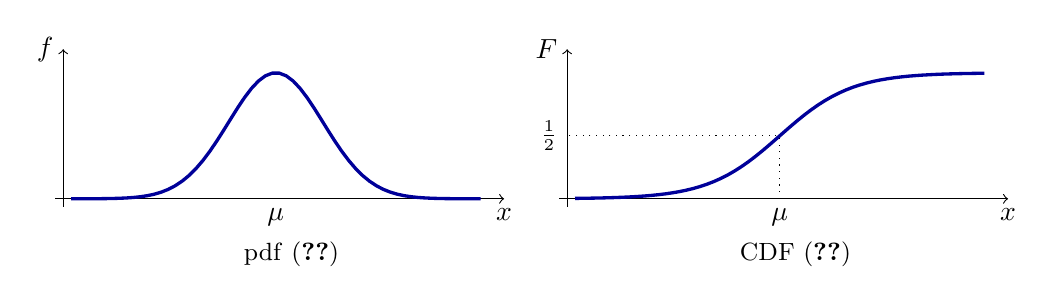
\begin{tikzpicture}[scale=1.0, domain=-2.6:2.6, samples=60]
\draw[->] (-2.8,0) -- (2.9,0) node[below] {$x$};
\draw[->] (-2.7,-0.1) -- (-2.7,1.9) node[left] {$f$};
\draw[very thick,color=blue!60!black]
  plot (\x, {1.6*exp(-\x*\x/0.72)});
\node[below] at (0,0) {$\mu$};
\node at (0.2,-0.7) {\small pdf \eqref{eq:pdf}};
\begin{scope}[xshift=6.4cm]
\draw[->] (-2.8,0) -- (2.9,0) node[below] {$x$};
\draw[->] (-2.7,-0.1) -- (-2.7,1.9) node[left] {$F$};
\draw[very thick,color=blue!60!black]
  plot (\x, {1.6/(1+exp(-2.2*\x))});
\draw[dotted] (0,0) -- (0,0.8) -- (-2.7,0.8);
\node[left] at (-2.7,0.8) {\small $\tfrac12$};
\node[below] at (0,0) {$\mu$};
\node at (0.2,-0.7) {\small CDF \eqref{eq:cdf}};
\end{scope}
\end{tikzpicture}
\end{center}

\begin{center}
\begin{tabular}{ll}
\toprule
Support & $\mathbb{R}$\\
Parameters & $\mu \in \mathbb{R}$, $\sigma^2 > 0$\\
Mean, median, mode & $\mu$\\
Variance & $\sigma^2$\\
Entropy & $\tfrac12 \log(2\pi e \sigma^2)$\\
Moment generating function & $\exp(\mu t + \tfrac12 \sigma^2 t^2)$\\
Fisher information & $I(\mu, \sigma^2) =
  \operatorname{diag}\bigl(1/\sigma^2,\; 1/(2\sigma^4)\bigr)$\\
Conjugate prior & $\mu$: Normal; $(\mu, \sigma^2)$:
  Normal--Inverse-Gamma\\
\bottomrule
\end{tabular}
\end{center}

\begin{proposition}[Exponential family form]
\label{prop:expfam}
With natural parameters $\eta = (\mu/\sigma^2,\, -1/(2\sigma^2))$ and
sufficient statistic $T(x) = (x, x^2)$,
\begin{equation}
  f(x; \mu, \sigma^2)
  \;=\; \exp\bigl(\eta^{\!\top} T(x) - A(\eta)\bigr),
  \qquad
  A(\eta) = \frac{\mu^2}{2\sigma^2} + \log(\sqrt{2\pi}\,\sigma),
\end{equation}
a full-rank two-parameter exponential family; the gradient of $A$ in
$\eta$ returns $\E[T] = (\mu,\, \mu^2 + \sigma^2)$.
\end{proposition}

\section{Statistics of the estimators}

Let $x_1, \dots, x_n$ be i.i.d.\ $\mathcal{N}(\mu, \sigma^2)$ and set
$\xbar = \tfrac1n \sum_i x_i$,
$\hat\sigma^2 = \tfrac1n \sum_i (x_i - \xbar)^2$.

\begin{proposition}[Sufficiency]
The likelihood depends on the data only through
$\bigl(\sum_i x_i,\, \sum_i x_i^2\bigr)$; by factorization this pair
(equivalently $(\xbar, \hat\sigma^2)$) is jointly sufficient.
\end{proposition}

\begin{proposition}[Properties of $\xbar$]
$\E[\xbar] = \mu$ and $\Var(\xbar) = \sigma^2/n = 1/(n I_{\mu\mu})$:
the sample mean is unbiased and attains the Cram\'er--Rao bound. As a
function of the complete sufficient statistic it is, by
Lehmann--Scheff\'e, the unique UMVUE of $\mu$. Moreover
$\xbar \sim \mathcal{N}(\mu, \sigma^2/n)$ \emph{exactly} at every $n$.
\end{proposition}

\begin{proposition}[Properties of $\hat\sigma^2$]
\label{prop:sighat}
The MLE variance is \emph{biased}:
\begin{equation}
  \E[\hat\sigma^2] \;=\; \frac{n-1}{n}\,\sigma^2,
  \label{eq:bias}
\end{equation}
since the sample mean absorbs one degree of freedom. The corrected
$s^2 = \tfrac{n}{n-1}\hat\sigma^2$ is unbiased (and UMVUE); both are
consistent, so the distinction vanishes as $n \to \infty$.
\end{proposition}

\begin{corollary}[Confidence interval]
An asymptotic $95\%$ interval for $\mu$ is
$\xbar \pm 1.96\, \hat\sigma/\sqrt{n}$ (exact with Student-$t$
quantiles in place of $1.96$).
\end{corollary}

\section{Maximum likelihood and maximum a posteriori estimation}

\subsection{Maximum likelihood}

\begin{theorem}[MLE]
\label{thm:mle}
The unique maximizer of the likelihood over
$(\mu, \sigma^2) \in \mathbb{R} \times (0, \infty)$ is
\begin{equation}
  \boxed{\;\hat\mu = \xbar, \qquad
  \hat\sigma^2 = \frac1n \sum_{i=1}^{n} (x_i - \xbar)^2.\;}
  \label{eq:mle}
\end{equation}
\end{theorem}

\begin{proof}
The log-likelihood is
\begin{equation}
  \ell(\mu, \sigma^2)
  \;=\; -\frac{n}{2}\log(2\pi\sigma^2)
        - \frac{1}{2\sigma^2}\sum_i (x_i - \mu)^2.
  \label{eq:loglik}
\end{equation}
For fixed $\sigma^2$, $\partial\ell/\partial\mu =
\tfrac{1}{\sigma^2}\sum_i (x_i - \mu) = 0$ gives $\mu = \xbar$
(a maximum: the second derivative $-n/\sigma^2 < 0$). Substituting
and differentiating in $v = \sigma^2$,
\begin{equation*}
  \frac{\partial \ell}{\partial v}
  \;=\; -\frac{n}{2v} + \frac{1}{2v^2}\sum_i (x_i - \xbar)^2 = 0
  \;\Longleftrightarrow\;
  v = \frac1n \sum_i (x_i - \xbar)^2,
\end{equation*}
with $\partial^2 \ell/\partial v^2 < 0$ at the stationary point.
\end{proof}

\subsection{Maximum a posteriori (known variance)}

\begin{proposition}[Conjugacy]
Fix $\sigma^2$ and let $\mu \sim \mathcal{N}(\mu_0, \tau^2)$. The
posterior is again normal.
\end{proposition}

\begin{theorem}[MAP]
\begin{equation}
  \boxed{\;\hat\mu_{\mathrm{MAP}}
  \;=\; \frac{\dfrac{n}{\sigma^2}\,\xbar + \dfrac{1}{\tau^2}\,\mu_0}
             {\dfrac{n}{\sigma^2} + \dfrac{1}{\tau^2}}\;}
  \label{eq:map}
\end{equation}
--- the precision-weighted average of data and prior.
\end{theorem}

\begin{proof}
Up to constants free of $\mu$, the log-posterior is
\begin{equation*}
  \log \pi(\mu \mid x_{1:n})
  \;=\; -\frac{1}{2\sigma^2}\sum_i (x_i - \mu)^2
        - \frac{(\mu - \mu_0)^2}{2\tau^2} + C.
\end{equation*}
Differentiating in $\mu$ and equating to zero,
\begin{equation*}
  \frac{1}{\sigma^2}\sum_i (x_i - \mu) - \frac{\mu - \mu_0}{\tau^2}
  = 0
  \;\Longleftrightarrow\;
  \frac{n}{\sigma^2}\,\xbar + \frac{\mu_0}{\tau^2}
  = \mu\Bigl(\frac{n}{\sigma^2} + \frac{1}{\tau^2}\Bigr),
\end{equation*}
which is \eqref{eq:map}; the second derivative
$-n/\sigma^2 - 1/\tau^2 < 0$ gives uniqueness. As $n \to \infty$ the
data precision $n/\sigma^2$ dominates and
$\hat\mu_{\mathrm{MAP}} \to \xbar$; as $\tau \to \infty$ (a flat
prior) it equals the MLE at every $n$.
\end{proof}

\section{Information theory}

\begin{definition}[Score and Fisher information]
The score of one observation is the gradient of $\log f$ in the
parameters,
\begin{equation}
  s(\mu, \sigma^2; x) \;=\;
  \Bigl(\frac{x - \mu}{\sigma^2},\;
  \frac{(x-\mu)^2 - \sigma^2}{2\sigma^4}\Bigr),
  \label{eq:score}
\end{equation}
with $\E[s] = 0$ and covariance the Fisher information matrix
$I(\mu, \sigma^2) = \operatorname{diag}(1/\sigma^2,\, 1/(2\sigma^4))$
--- diagonal: location and scale carry independent information.
\end{definition}

\begin{definition}[Entropy and KL divergence]
$H = \tfrac12\log(2\pi e\sigma^2)$, and for two Gaussians
\begin{equation}
  \mathrm{KL}\bigl(\mathcal{N}(\mu_1,\sigma_1^2) \,\|\,
  \mathcal{N}(\mu_2,\sigma_2^2)\bigr)
  \;=\; \log\frac{\sigma_2}{\sigma_1}
  + \frac{\sigma_1^2 + (\mu_1 - \mu_2)^2}{2\sigma_2^2}
  - \frac12 \;\ge\; 0.
  \label{eq:kl}
\end{equation}
\end{definition}

\begin{remark}
Minimizing the average negative log-likelihood over
$(\mu, \sigma^2)$ minimizes the cross-entropy between the empirical
distribution and the model; the fitted Gaussian is the
information projection of the data onto the family. The Jeffreys
prior $\pi \propto \sqrt{\det I} \propto 1/\sigma^3$ (or
$1/\sigma$ for known mean) is the scale-invariant reference prior.
\end{remark}

\section{Numerical solution by stochastic gradient descent}

To free both constraints, reparameterize $\sigma = e^{s}$ and
minimize the average negative log-likelihood in $(\mu, s) \in
\mathbb{R}^2$:
\begin{equation}
  F(\mu, s) \;=\; \frac12\log(2\pi) + s
  + \frac{1}{2e^{2s}}\,\overline{(x - \mu)^2}.
\end{equation}

\begin{proposition}[Gradients]
\begin{equation}
  \boxed{\;
  \frac{\partial F}{\partial \mu} = \frac{\mu - \xbar}{e^{2s}},
  \qquad
  \frac{\partial F}{\partial s}
  = 1 - \frac{\overline{(x-\mu)^2}}{e^{2s}},\;}
  \label{eq:grad}
\end{equation}
with per-sample versions replacing the averages by single samples.
\end{proposition}

\begin{proof}
$\partial F/\partial \mu = \tfrac{1}{2e^{2s}} \cdot
\overline{2(\mu - x)} = (\mu - \xbar)/e^{2s}$. For $s$: the middle
term differentiates to $1$; by the chain rule
$\partial (e^{-2s})/\partial s = -2e^{-2s}$, so the last term gives
$-\overline{(x-\mu)^2}/e^{2s}$. At a stationary point
$\mu = \xbar$ and $e^{2s} = \overline{(x-\xbar)^2}$ --- the MLE
\eqref{eq:mle}, recovered by invariance through
$\sigma = e^{s}$.
\end{proof}

SGD iterates these per-sample gradients over shuffled passes;
constant step sizes leave the iterates in a noise ball, and the
Polyak--Ruppert average of the final pass is reported. Automatic
differentiation of the same objective reproduces \eqref{eq:grad}
exactly, asserted by the companion program on an identical schedule.

\section{Numerical verification}

\texttt{gaussian.py} ($\mu = 2$, $\sigma = 1.5$, $n = 5000$, seed 7):

\begin{center}
\begin{tabular}{lll}
\toprule
Claim & Reference & Measured\\
\midrule
Moments of the sample & \S1 & mean, var within $10^{-2}$\\
$\E[\hat\sigma^2] = \tfrac{n-1}{n}\sigma^2$ &
  Prop.~\ref{prop:sighat} & factor $0.800$ at $n{=}5$ (theory $0.8$)\\
MLE vs.\ grid maximization & Thm.~\ref{thm:mle} & agree to $10^{-3}$\\
Flat prior: MAP $\to$ MLE & Thm.~2 & exact as $\tau \to \infty$\\
Small-$n$ MSE, MAP vs.\ MLE & \eqref{eq:map} & MAP smaller\\
Score moments & \eqref{eq:score} & $\E[s] \approx 0$,
  $\mathrm{Cov} \approx I$\\
Polyak vs.\ closed form & \eqref{eq:grad} & within $10^{-2}$\\
Hand SGD vs.\ autograd & \S5 & max gap $< 10^{-10}$\\
\bottomrule
\end{tabular}
\end{center}

\end{document}
